\section{Software}
\label{sec:chapterexample}

\subsection{Programmiersprachen}
Das System besteht aus mehrere Programme und Dienste. Für die Entwicklung werden folgende Programmiersprachen eingesetzt:
\begin{itemize}
	\item Java
	\item Javascript
	\item PHP
\end{itemize}
Im Verbindung mit PHP kommt natürlich die Markup-Languages HTML5/CSS, welche für die graphische Darstellung der Webapplikationen notwendig ist.

\subsubsection{Java}
\label{kap:java}
Alle Dienste die Serverseitig und ohne Interaktion mit dem Enduser ausgeführt werden, werden in Java programmiert. Als stark typisierte und Objektorientierte Programmiersprache eignet sich Java für dieses Projekt. Für Java sind auch unzählige Libraries verfügbar, insbesondere für die Hardware Steuerung der Raspberry Pi. Eine zweite Variante wäre Python gewesen, die auch das Raspberry sehr gut unterstüzt. Python ist aber zu wenig typisiert und für eher kleinere Softwarestücke gedacht.

\subsubsection{PHP/Javascript}
Die Enduser Applikation sowohl auch die Applikation bei der Aussensprechstelle werden Web-Applikationen sein. Dies ermöglicht eine schnelle und zeitgemässe Softwareentwicklung. Für dieses Projekt ist die System-Eingriffstiefe von Webapplikationen jedenfalls ausreichend. Es muss lediglich Zugriff auf Mikrofon, Lautsprecher und Kamera garantiert werden. Ein weiteres Punkt zugunsten einer Webapplikation ist die Cross-Plattform Kompatibilität. 
\\
Aus diesem Grund haben wir uns für PHP (Objektorientiert) im Kombination mit Javascript/HTML/CSS Entschieden. Eine zweite Variante wäre Java EE gewesen. Java EE eignet sich aber vor allem für grosse Softwarelösungen und bietet als gesamten Framework vieles mehr als was dieses Projekt benötigt. 
\\
\subsubsection{PHP Framework: Laravel}
Für die Entwicklung der Webapplikationen wird Laravel als PHP Framework eingesetzt. Laravel ist ein Open-Source PHP Web-Application-Framework, die sich für kleine bis zu mittelgrosse Projekte eignet. Laravel beruht auf dem Modell-View-Controller-Muster und ermöglicht eine Objektorientierte Programmierung in PHP.

\subsection{Software-Ecosystem}
Das System besteht aus mehrere Hardware- und Softwarekomponenten die zusammenarbeiten müssen (\seeref{fig:echosystem}). Die Kommunikation zwischen den Knoten ist von TLS immer gewährleistet. Die einzelne Komponente werden in den nächsten Kapiteln genauer beschrieben.

\begin{figure}[htb!]
	\begin{center}
		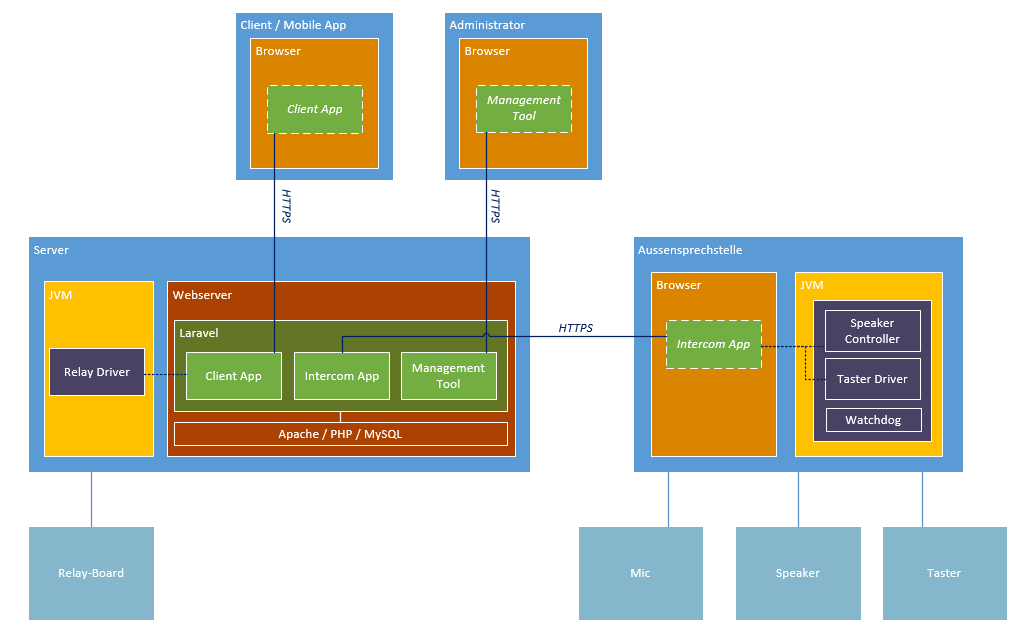
\includegraphics[width=1\textwidth]{ecosystem}
		\caption[Software / Hardware Ecosystem]{Software / Hardware Ecosystem}
		\label{fig:echosystem}
	\end{center}
\end{figure}

Die Software wird in zwei Gruppen unterteilt. Einerseits gibt es alle Dienste/Services \textit{(Violett)} die Lokal ausgeführt werden und quasi das Backend des Systems darstellen (\seeref{kap:dienste}). 
\\
Die zweite Gruppe beinhaltet die Webapplikationen \textit{(Grün)}, die eine GUI besitzen und für die Interaktion mit dem System gedacht sind. Darunter zählen die Client-App für den Bewohner, die Applikation bei der Aussensprechstelle wo die Bewohner angezeigt werden und das Management Tool. (\seeref{kap:webapp})
\\
Die Audio-Kommunikation zwischen die Aussensprechstellen und die Client-Apps wird mithilfe von WebRTC realisiert. Diese hat eine gewisse Komplexität und wird in ein eigenes Kapitel (\seeref{kap:webrtc}) behandelt.

\subsection{Dienste}
\label{kap:dienste}


\subsubsection{Keymapper}
Die Aussensprechstelle wird durch 3 Schalter bedient. Die Aufgabe des Keymappers besteht darin, bei einem Tastendruck eine Aktion auf der Aussensprechselle ausgeführt wird. Die drei Schalter wurden an GPIO Pins des Raspberry PI angeschlossen. Wie im \cref{kap:java}
beschrieben wurde, wird Java eingesetzt. 
\\
Die ursprüngliche Idee war der Keymapper als Daemon im Hintergrund laufen zu lassen. Diese würde der Vorteil haben das der Daemon mittels run, stop und restart stabil gesteuert werden könnte. Da die eingesetzte java Library zum laufen zwingend ein X server benötigt, wurde der Keymapper im Init level 5 wo auch der X Server ausgeführt. Die Ausführung der Software ergibt in diesem Fall eine Fehlermeldung da die X Server noch nicht vollständig initialisiert ist. 
Das Problem lag darin das per Definition ein Daemon Benutzerunabhängig ist. Somit steht der Library die auf dem X Server zugreift die wiederum Benutzerspezifisch ist, in Konflikt mit der Definition. 
\\
Die Desktop-Umgebung LXDE welche von Raspbian verwendet wird, bietet ein Autostart welche die Keymapper nach dem Initialisierung des X Server ausführt.

\subsubsection{Speaker Controller}
...
\subsubsection{Relay Controller}
...
\subsubsection{Watchdog}
...

\subsubsection{Signaling Server}
Der Signaling-Server ist ein bestandteil von WebRTC und wird in ein eigenes Kapitel ausführlich beschrieben (\seeref{kap:webrtc}).


\subsection{Webapplikationen}
\label{kap:webapp}


\subsubsection{Client Webapplikation}
Der Bewohner muss über eine Applikation verfügen, die auf dem Tablet oder Handy ausführbar sein muss. Mithilfe dieser App muss der Enduser folgendes können: Sich mit alle Aussensprechstellen verbinden können, ein Video Signal von der Kamera aller Eingänge erhalten, alle Türe öffnen und mit der Person bei der Türe über die Anlage kommunizieren können.
\\
\begin{figure}[htb!]
	\begin{center}
		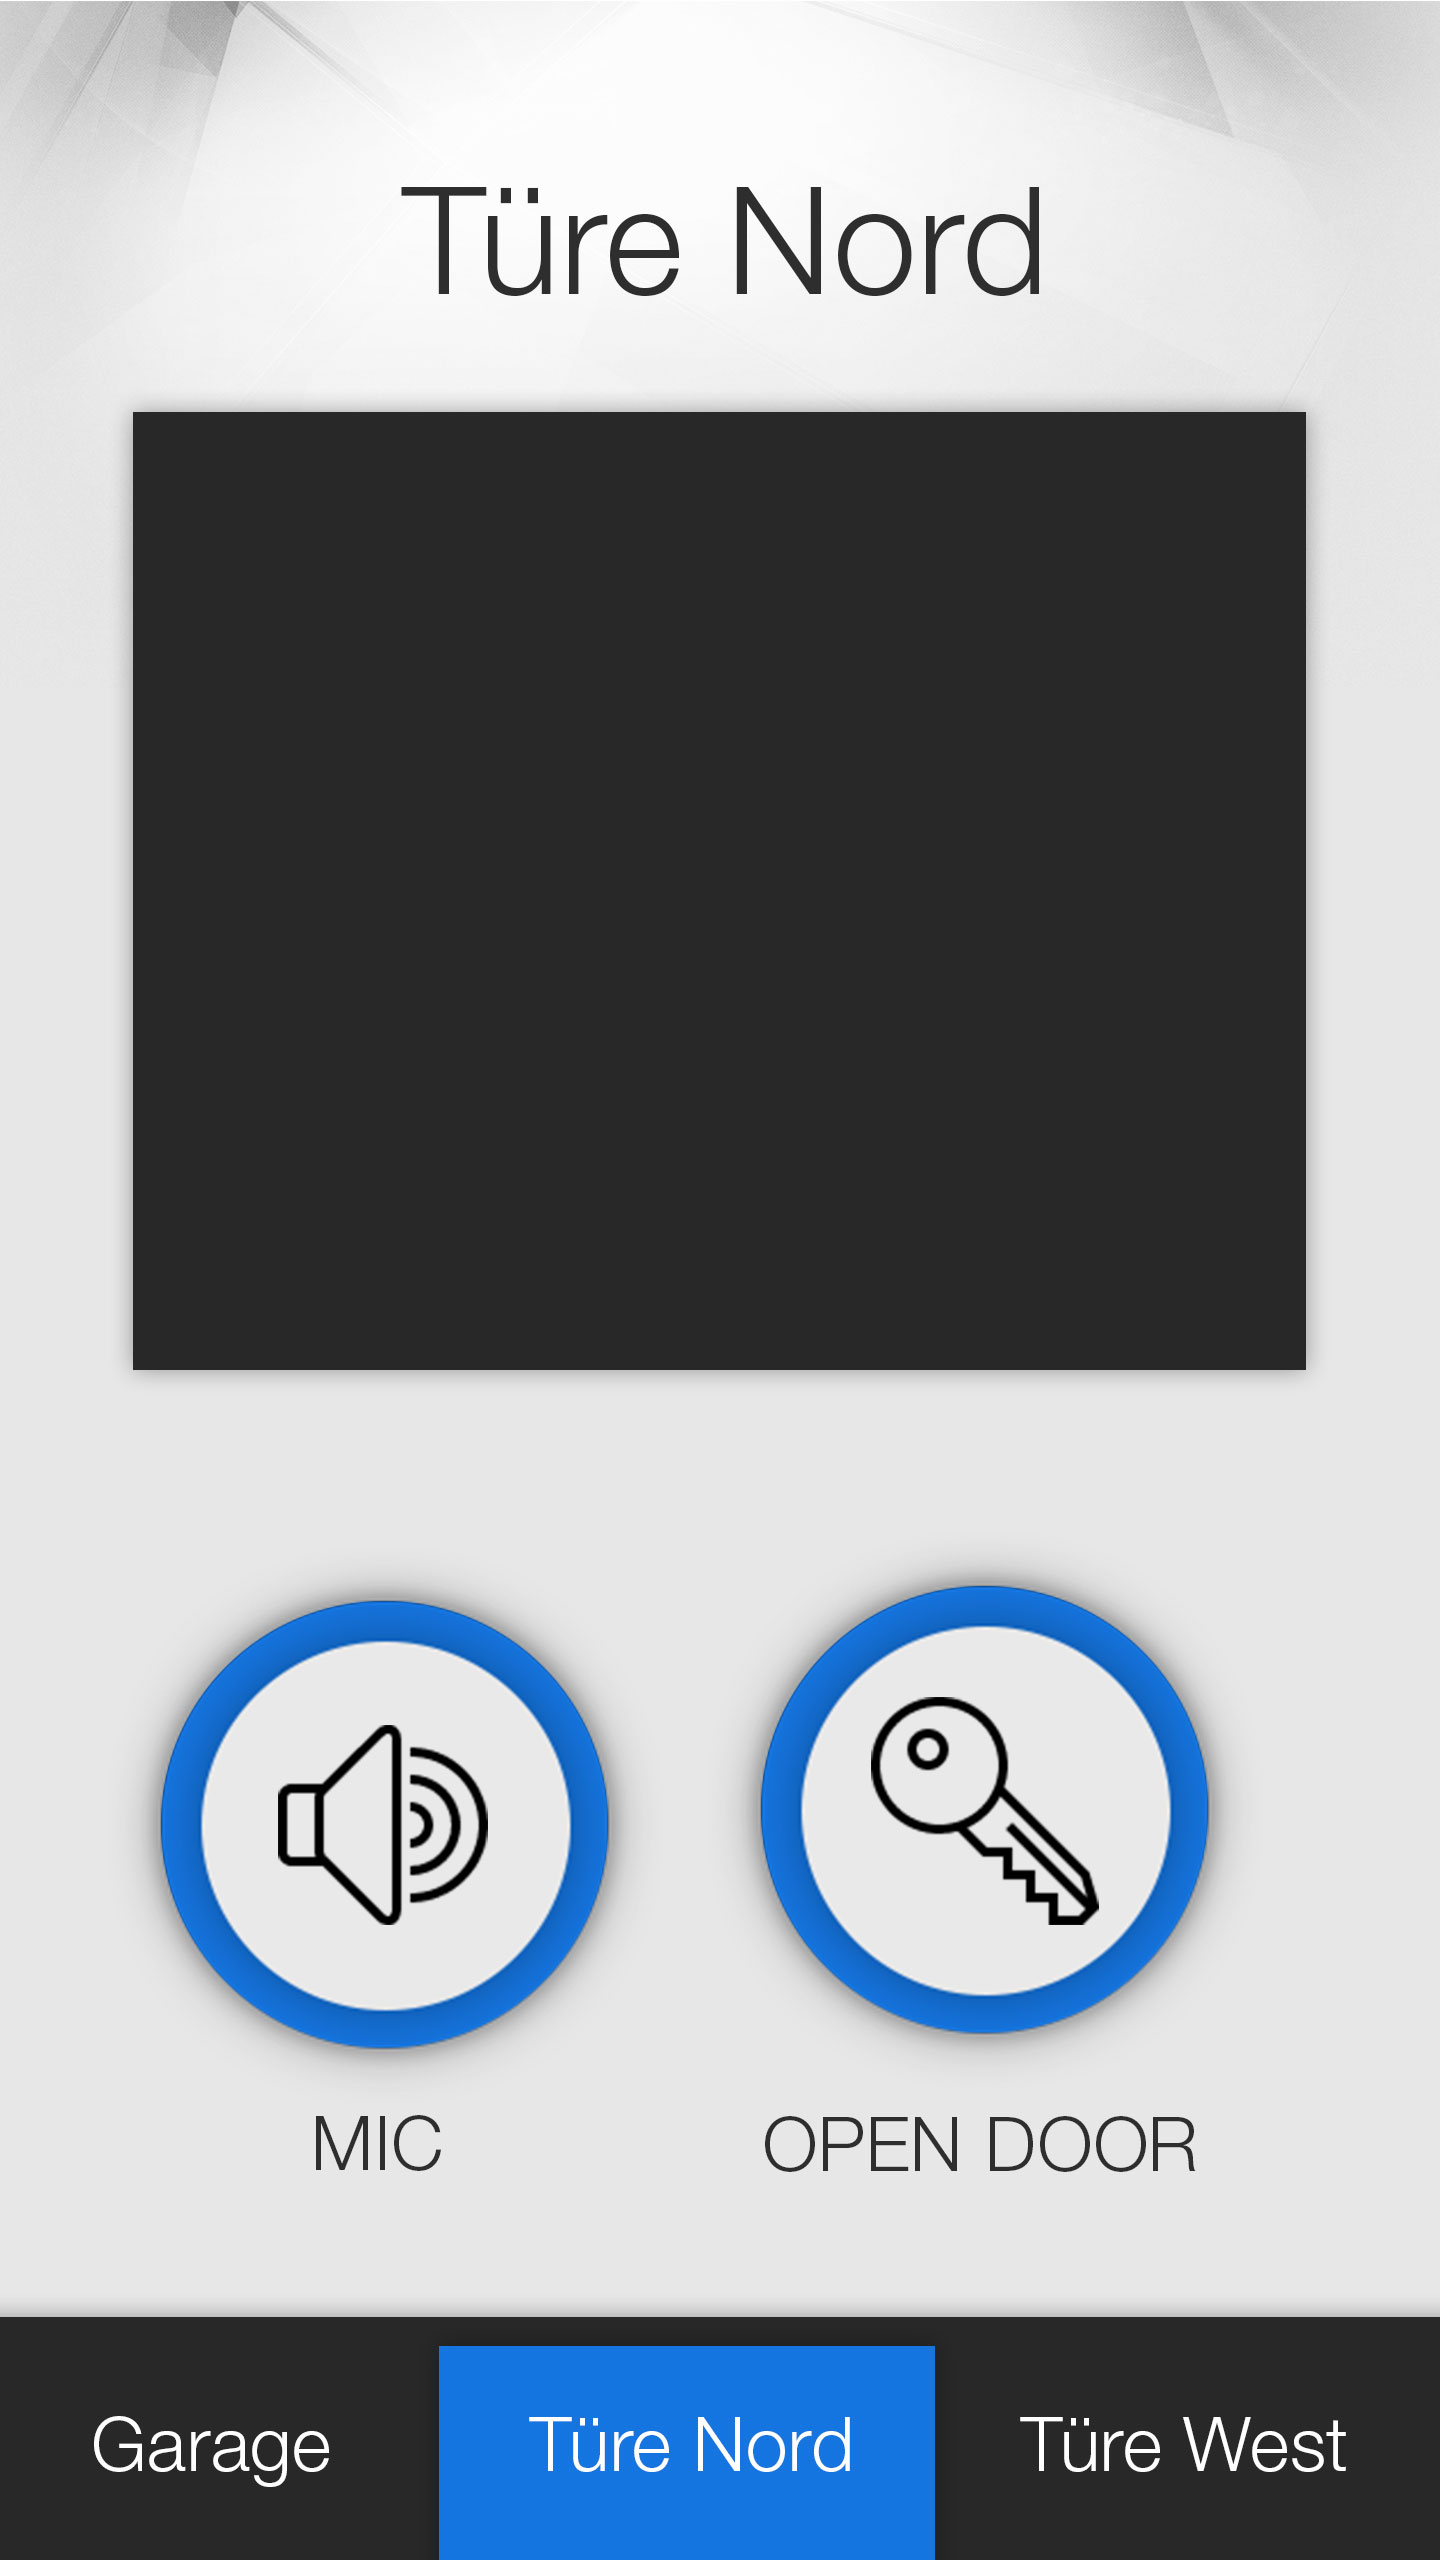
\includegraphics[width=0.35\textwidth]{clientDemo}
		\caption[Design der Client-Webapp]{Design der Client-Webapp}
		\label{fig:clientDemo}
	\end{center}
\end{figure}
\\
Die \cref{fig:clientDemo} zeigt das Design für diese Webapplikation. Hier gezeigt ist die Smartphone Version. Dank ein Responsive-Design wird die selbe Applikation auch auf andere Geräte wie z.B. Tablets oder Computers passend angezeigt.
\\ 
Bei der Design-Entwurf standen Übersichtlichkeit und Benutzerfreundlichkeit im Vordergrund. Aus diesem Grund werden die Tasten für die Audio-Kommunikation und für die Öffnung der Türe gross Angezeigt. Das Videostream von der ausgewählte Türe wird sofort angezeigt und benötigt keine weitere Interaktion. 


\subsection{WebRTC}
\label{kap:webrtc}

\newpage